\documentclass[../main.tex]{subfiles}
\graphicspath{{\subfix{../figures/}}}

\begin{document}

\chapter{{DiffFracQuant: Bayesian Model for the Detection of Differential Fractionation}}

\section{Chapter 5 Introduction}

% https://www.nature.com/articles/s41580-021-00356-8

% Poor data sets
% https://www.ncbi.nlm.nih.gov/geo/query/acc.cgi?acc=GSE99304
% https://www.ncbi.nlm.nih.gov/geo/query/acc.cgi?acc=GSE99170

% https://www.encodeproject.org/experiments/ENCSR000COR/

% https://www.encodeproject.org/experiments/ENCSR000COQ/

% https://www.encodeproject.org/experiments/ENCSR000CPO/

Localisation of RNA populations to specific sub-cellular compartments is a widely implemented mechanism to regulate gene expression.
Focusing localisation machinery on mRNA transcripts rather than proteins is more energy efficient as one mRNA transcript can lead to the translation of hundreds of proteins.
Rapid changes in gene expression in response to stimuli such as heat stress can be achieved by chaperoning surplus mRNA transcripts into stress granules where they cannot be translated.
In plant and animal cells, microRNA (miRNA), long non-coding RNA (lncRNA) and small interfering RNA (siRNA) contribute to gene expression regulation through splicing, degradation or translation pathways specific either to the nucleus or cytoplasm.

Several RNA-Seq assays have been developed to isolate and compare RNA populations in different sub-cellular compartments.
Fractions of mRNA from organelles of different weights can be separated by centrifuging lysed cells. 
Centrifugation using a sucrose gradient or by repeating the process on the supernatent under increasing speeds can separate multiple fractions within on experiment.
Alternatively, fractions of freely floating vs protein bound mRNA can be separated by orthogonal organic phase separation. 
Despite the development of multiple fractionation-based RNA-Seq assays, there are a limited number of statistical methods to analyse them.

RNASeq datasets need to be normalised to remove batch effects and flow cell dependent biases (often introduced during reverse transcription and amplification). 
Differential expression analysis is easily confounded by RNASeq biases.
To be able to compare samples across RNA-seq runs users need to be able to remove biases that changes from run to run. 
For example, the amplification of reads from each lane of a RNA-seq machine varies significantly. 
Other amplification biases can be introduced, the shotgun method of short read sequencing means the number of reads per gene will be proportional to the length of that gene. 
In addition elongation biases between the nucleotides can change the amplificiation ratio of genes.
Certain gene with high GC content may not be amplified as well because they bind too tightly for the melting stage to occur efficiently. 
Raw reads are rarely used as the measure of expression between samples and between genes. Instead, they are normalised either by internal methods or by external controls such as spike-in samples. 

Internal normalisation commonly consists of converting raw reads into transcripts per million or reads per million.
It can been widely reported at the read per million method has significant biases and should not be used. 
However, transcripts per million account for the total read variation between runs and the gene length biases. However, dividing by total reads does leave TPM counts vunerable to being dominated by the behaviour of a few highly expressed genes.
Since there is a large order of magnitude between expression across an organisms genome, gene that are expressed on the order of $10^4$ transcripts per cell will contribute more to the total reads compared to transcript that only occur once or twice. 
If the experiments significant change the expression of the highly expressing genes but the users is mostly interested in the behavour of the lowly expressing genes, comparing TPM may confound expression patterns. Neither method attempts to deal with GC biases. Alternatively, an external control of known volumes of synthetic RNA can be introduced with differing GC content and lengths. 
The comparison of these RNA levels after being amplified in the RNA-seq assay can discover biases in transcript length, total read and GC content.
A rigorous method for using this information to normal counts across the genome has not be developed as error in spike-in volumes are very common and obscure predictions expected reads post-sequencing.

Median based techniques such as those used by DESeq attempts to find the behaviour of the most average gene across the condition.
This is combined with shrinkage methods to reduce variance in lowly expressed genes.
Under the assumption that most genes do not express differently across genes then the change in the most average gene must be down to biases.
This assumption breaks down in cases where the majority of gene are expected to have different expression across RNA-Seq samples. 
However, the normalisation method in DESeq2 assumes the majority of genes are expressed at similar levels across conditions. 
It uses this assumption to share dispersion information across genes so that gene-wise shrinkage estimates can be determined to account for biases. 
In assays that extract RNA from different fractions, changes in abundance across the entire transcriptome can be expected. 
This invalidates DESeq2’s assumptions.
However, the fact that fractionation assays consist of small samples from a larger pool provides an alternative method for normalisation.


The work here outlines an alternative way of normalising RNA-Seq data sets and comparing fractions using the additional information that can be gathered in measure subsets of a complete cell.
This will enable even more seditive comparisons of transcript localisation across conditions and cell types.
Diff Frac: Normalisation of RNA-Seq data to enable comparison across experiments remains a non-trivial task. 
Modelling errors using Bayesian statistical models and implementing quality experimental design can overcome many issues.



\section{Chapter 5 Results}

\subsection{Bayesian Hierarchical Model}

\begin{figure}
     \centering
     \begin{subfigure}[b]{0.4\textwidth}
     \centering
     \tikz{
        % Nodes
        \node[obs]                                   (N-t)   {$N^{Tot}_{grc}$}; %
        \node[obs, left=1 of N-t]                    (N-s)   {$N^{Sup}_{grc}$}; %
        \node[obs, right=1 of N-t]                   (N-p)   {$N^{Pel}_{grc}$}; %
        \node[latent, below=1 of N-s, xshift=0.6cm]  (l-s)   {$\lambda^{Sup}_{gc}$}; %
        \node[latent, below=1 of N-p, xshift=-0.55cm] (l-p)   {$\lambda^{Pel}_{gc}$}; %
        \node[latent, below=3 of N-t, yshift=-0.2cm] (p-t)     {$\phi^{Tot}$}; %
        \node[latent, below=3 of N-s, yshift=-0.2cm, xshift=0.15cm] (p-s)     {$\phi^{Sup}$}; %
        \node[latent, below=3 of N-p, yshift=-0.2cm, xshift=-0.15cm] (p-p)     {$\phi^{Pel}$}; %
        \node[latent, above=1 of N-t] (a-t)     {$a^{Tot}_{cr}$}; %
        \node[latent, above=1 of N-s, xshift=-0.3cm] (a-s)     {$a^{Sup}_{cr}$}; %
        \node[latent, above=1 of N-p, xshift=0.3cm] (a-p)     {$a^{Pel}_{cr}$}; %
        \node[latent, above=1 of a-t, yshift=-0.3cm] (alpha-p)     {$\alpha$}; %
        \node[latent, below=0.6 of p-t] (sigma-t)     {$\sigma^2$}; %
        
        
        % Connections
        \edge {a-t} {N-t} ; %
        \edge {a-s} {N-s} ; %
        \edge {a-p} {N-p} ; %
        \edge {p-t} {N-t} ; %
        \edge {p-s} {N-s} ; %
        \edge {p-p} {N-p} ; %
        \edge {l-s} {N-t, N-s} ; %
        \edge {l-p} {N-t, N-p} ; %
        \edge {alpha-p} {a-p, a-s} ; %
        \edge {sigma-t} {l-s, l-p} ; %
        
        % plate
        \plate {rep} {(N-t)(N-p)(N-s)(a-t)(a-p)(a-s)} {$Rep$}
        \plate {gene} {(l-p)(l-s)(N-t)(N-p)(N-s)(rep-caption)} {$Gene$}
        \plate {con} {(N-t)(N-p)(N-s)(gene)(rep)} {$Con$}
    }
    \end{subfigure}
     \hfill
     \begin{subfigure}[b]{0.57\textwidth}
     \centering
     \begin{align*}
        N^{Tot}_{grc} & \sim  negbin(a^{Tot}_{cr}(e^{\lambda^{Sup}_{gc}} + e^{\lambda^{Pel}_{gc}}), \phi^{Tot})\\
        N^{Pel}_{grc} & \sim  log\_negbin(a^{Pel}_{cr}+\lambda^{Pel}_{gc}, \phi^{Pel})\\
        N^{Sup}_{grc} & \sim  log\_negbin(a^{Sup}_{cr}+\lambda^{Sup}_{gc}, \phi^{Sup})\\
        &\\
        \lambda^{Sup}_{gc}, \lambda^{Pel}_{gc} &\sim normal(\mu, \sigma^2)\\
        \mu &\sim normal(7,2)\\
        \sigma^2&\sim normal(2,1)\\
        &\\
        \phi^{Tot}, \phi^{Sup}, \phi^{Pel}&\sim normal(100,10)\\
        a^{Tot}_{cr}&\sim normal(10, 0.1)\\
        a^{Sup}_{cr}, a^{Pel}_{cr}&\sim normal(\alpha, 0.1)\\
        \alpha&\sim normal(0, 0.5)
    \end{align*}
     \end{subfigure}
     \caption[Overview of DiffFracQuant Model.]{\textbf{Plate diagram summarising the Bayesian hierarchical model behind DiffFracQuant.} Shaded circles represent observed variables, in this case the unnormalised RNA-Seq transcript counts, and white circles represent latent variables learnt by the model. Circles placed within a square plate have separate random variables for each possible value associated with that plate, i.e. the $a^{Sup}$ circle is within the Rep plate and Con plate as there is a $a^{Sup}$ for each replicate and condition.}
\end{figure}

\subsection{Test Data Sets}
The performance of DiffFracQuant compared to DESeq2 is tested using three data sets: two experimental and one simulated.
The simulated data set consists of 300 genes with total transcript counts, $X^{Tot}$, sampled from a lognormal distribution to simulate the range of gene expressions in an RNA-Seq data set.
The ratio of transcripts between fraction A and B for each gene, $\gamma$, is sampled from a beta distribution to give a range of effect sizes.
The parameters of the beta distribution were set to simulate three regimes: all gene are randomly allocated a fraction, most genes have a marginal bias towards fraction B, and the majority of transcripts are in fraction B but transcripts from a specific subset of genes are found in fraction A.
Noise typically associated with RNA-Seq data set is introduced to the ideal genewise transcript counts by sampling from a negative binomial with the ideal values as its mean to create the training data, $N^{A}$, $N^{B}$ and $N^{Tot}$.
Three data points are sampled for each gene in each fraction and condition to represent three replicates.
Finally, a RNA-Seq run specific parameter, $\alpha$, is introduce to represent the varying total reads expected from every replicate, condition and fraction.

$$X^{Tot}_g \sim lognormal(\mu, \sigma^2)$$
$$N^{A}_{grc} \sim negbin(\gamma_{gc}\alpha^{A}_{rc}X^{Tot}_g,\phi)$$
$$N^{B}_{grc} \sim negbin((1-\gamma_{gc})\alpha^{B}_{rc}X^{Tot}_g,\phi)$$
$$N^{Tot}_{grc} \sim negbin(\alpha^{Tot}_{rc}X^{Tot}_g,\phi)$$
$$\alpha \sim uniform(min=0.5, max=3)$$
$$\gamma_{gc}\sim beta(a_c,b_c)$$

The first experimental data set comes from the Encyclopedia of DNA Elements (ENCODE) consortium. 
The data set consists of total, nuclear and cytoplasmic poly(A) RNA transcripts from a human GM12878 lymphoblastoid cell line.
The fractions were separated using centrifugation and include two bioreps, Figure \ref{fig:fractionation-datasets}B.
The reads were already aligned to the hg38 human reference genome and counted by the RSEM software following the standard ENCODE analysis pipeline.
The second experimental data set is from a paper investigating the formation of heat-induced stress granules in \textit{Saccharomyces} cerevisiae.
RNA transcripts held in stress granules were pelleted by 18,000g centrifugation and are available alongside transcripts freely floating in the supernatant and transcripts sampled before centrifugation across two bioreps, Figure \ref{fig:fractionation-datasets}C.
The reads were already aligned to the S288C reference genome (release R64-2-1) and counted used the STAR aligner.
The \textit{Saccharomyces} data set also includes a deletion strain in each of the three temperatures, but it is not used here. 

\begin{figure}[h]

{\centering 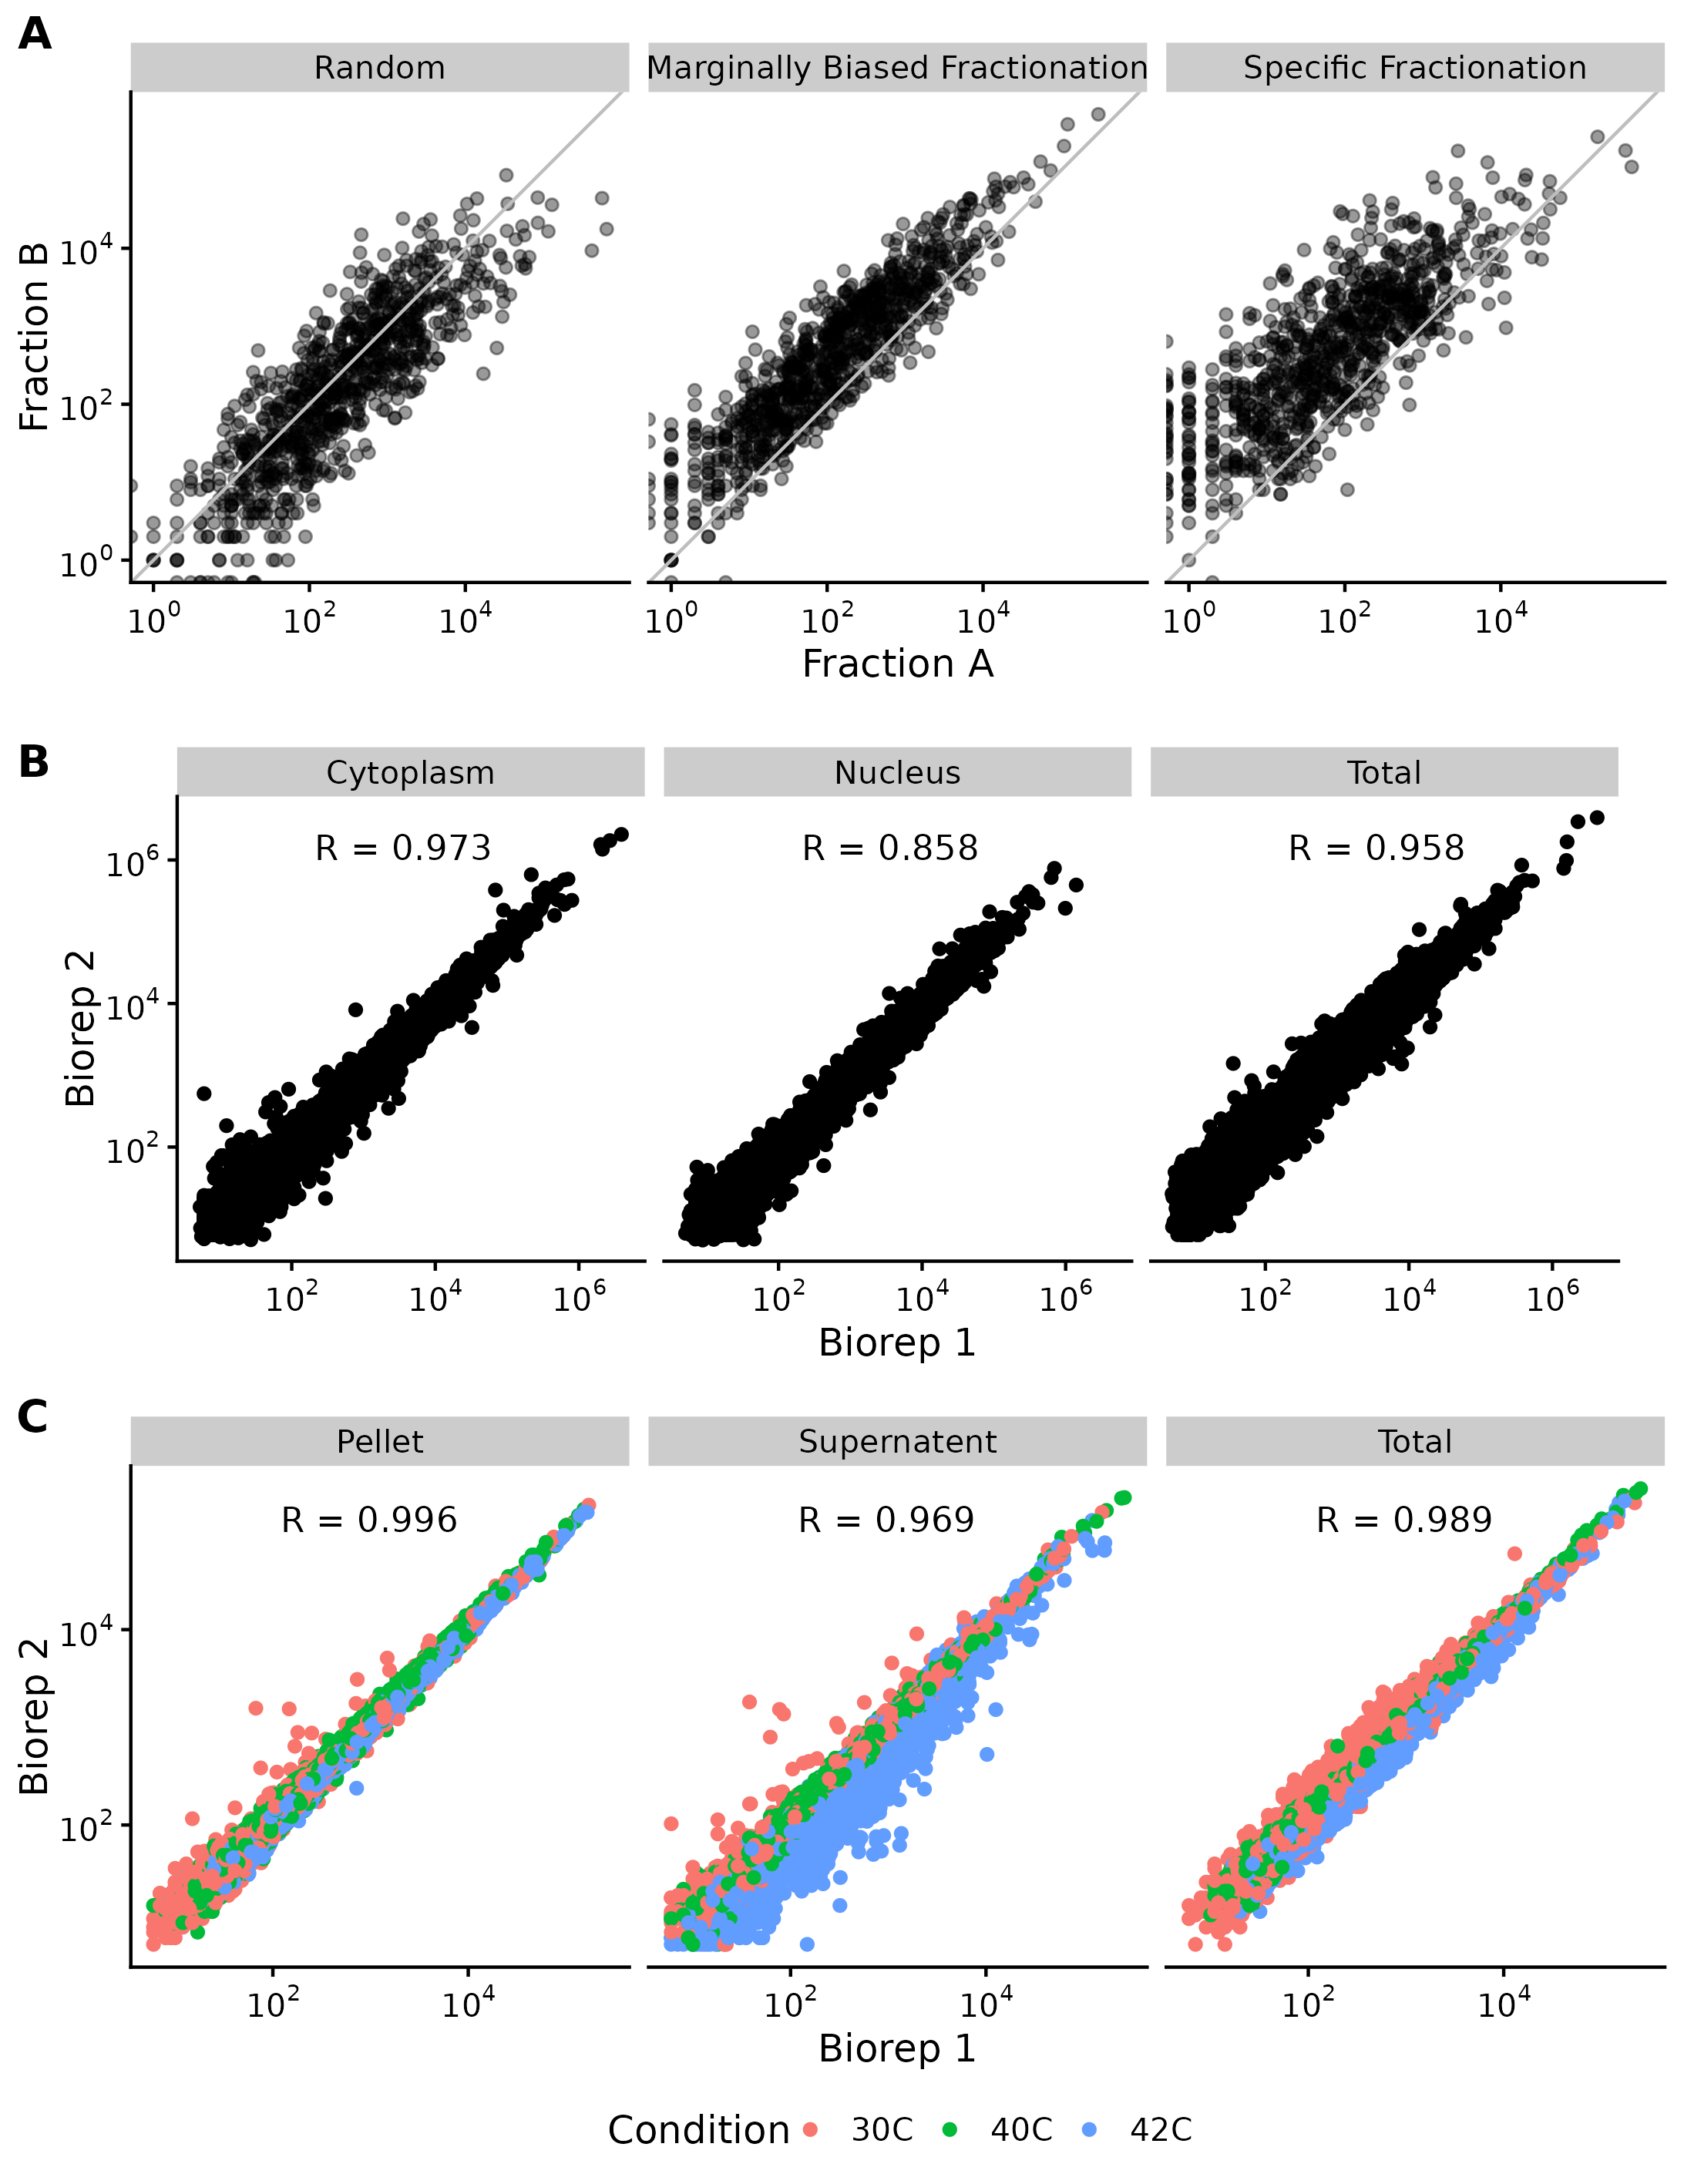
\includegraphics[width=0.8\linewidth]{figures/fractionation_dataset_summary.png} 

}

\caption[Overview of fractionation data sets.]{\textbf{Overview of the two experimental and one simulated data sets used in this study.} \textbf{(A)}  Simulated mRNA transcript counts between two fractions in three regimes: all gene are randomly allocated a fraction, most genes have a marginal bias towards fraction B, and the majority of transcripts are in fraction B but transcripts from a specific subset of genes are found in fraction A. 
\textbf{(B)} Correlation between two biological replicates of nuclear vs cytoplasmic mRNA transcript counts in a human lymphoblastoid cell line from the ENCODE project \parencite{Dunham2012}. \textbf{(C)} Correlation between two biological replicates of mRNA transcript counts in heat shock induced stress granules vs freely floating in \textit{Saccharomyces} cerevisiae cells. The dataset includes three temperature conditions: optimal 30C, mild 40C heat shock, and extreme 42C heat shock  \parencite{Iserman2020}.} \label{fig:fractionation-datasets}
\end{figure}

\subsection{Quantifying Fractionation in the Simulated Data Set}

The three replicates of noisy $N^{Tot}$, $N^{A}$ and $N^{B}$ counts from each regime of the simulated data set are used to train the DiffFracQuant model.
1000 samples of $\lambda^{A}$ and $\lambda^{B}$ are taken from the posterior distribution after a 1000 iteration burn-in.
A gene is considered to be significantly localised to fraction B if 97.5\% of the $\lambda^{B}$ samples are greater than $\lambda^{A}$ for that gene in that regime.
DiffFracQuant is compared to the results from DESeq2 trained on $N^{A}$ and $N^{B}$ counts.
DESeq2 is used according to the standard workflow outlined in its documentation.
The workflow includes the determination of normalisation factors, estimation of dispersion and calculation of significance using a Wald test. 

The log$_2$ ratio of transcript counts between the two fractions as calculated by DESeq2 and DiffFracQuant were compared to the log$_2$ ratio of noiseless counts in the simulated data set, $\gamma/(1-\gamma)$, Figure \ref{fig:simulated-data-results}A.
The correlation between predicted log$_2$ ratio and ground truth is greater than 0.98 for both methods in all regimes. 
However, as the ratio of transcript between fractions for each gene changes from a random distribution to being predominately localised in fraction A the disparity between the models develops. 
The log$_2$ ratios from DiffFracQuant consistently match the ground truth across all conditions and magnitudes.
The log$_2$ ratios from DESeq2 shift down below the ground truth as the normalisation factor begins to include some of the change in total transcriptome level.
This behaviour is reflected in the detection of significant difference in transcript abundance between the two fractions.
Across all genes, DESeq2 has a larger false discovery rate (FDR) in the marginal and specific regimes than DiffFracQuant.
Although DESeq2 does have a marginally better FDR in the random regime its true positive rate (TPR) is notably less than DiffFracQuant.
This behaviour is replicated over the 60 least abundant genes and the 60 genes with the smallest change between the conditions, Figure \ref{fig:simulated-data-results}B.

\begin{figure}[h]

{\centering 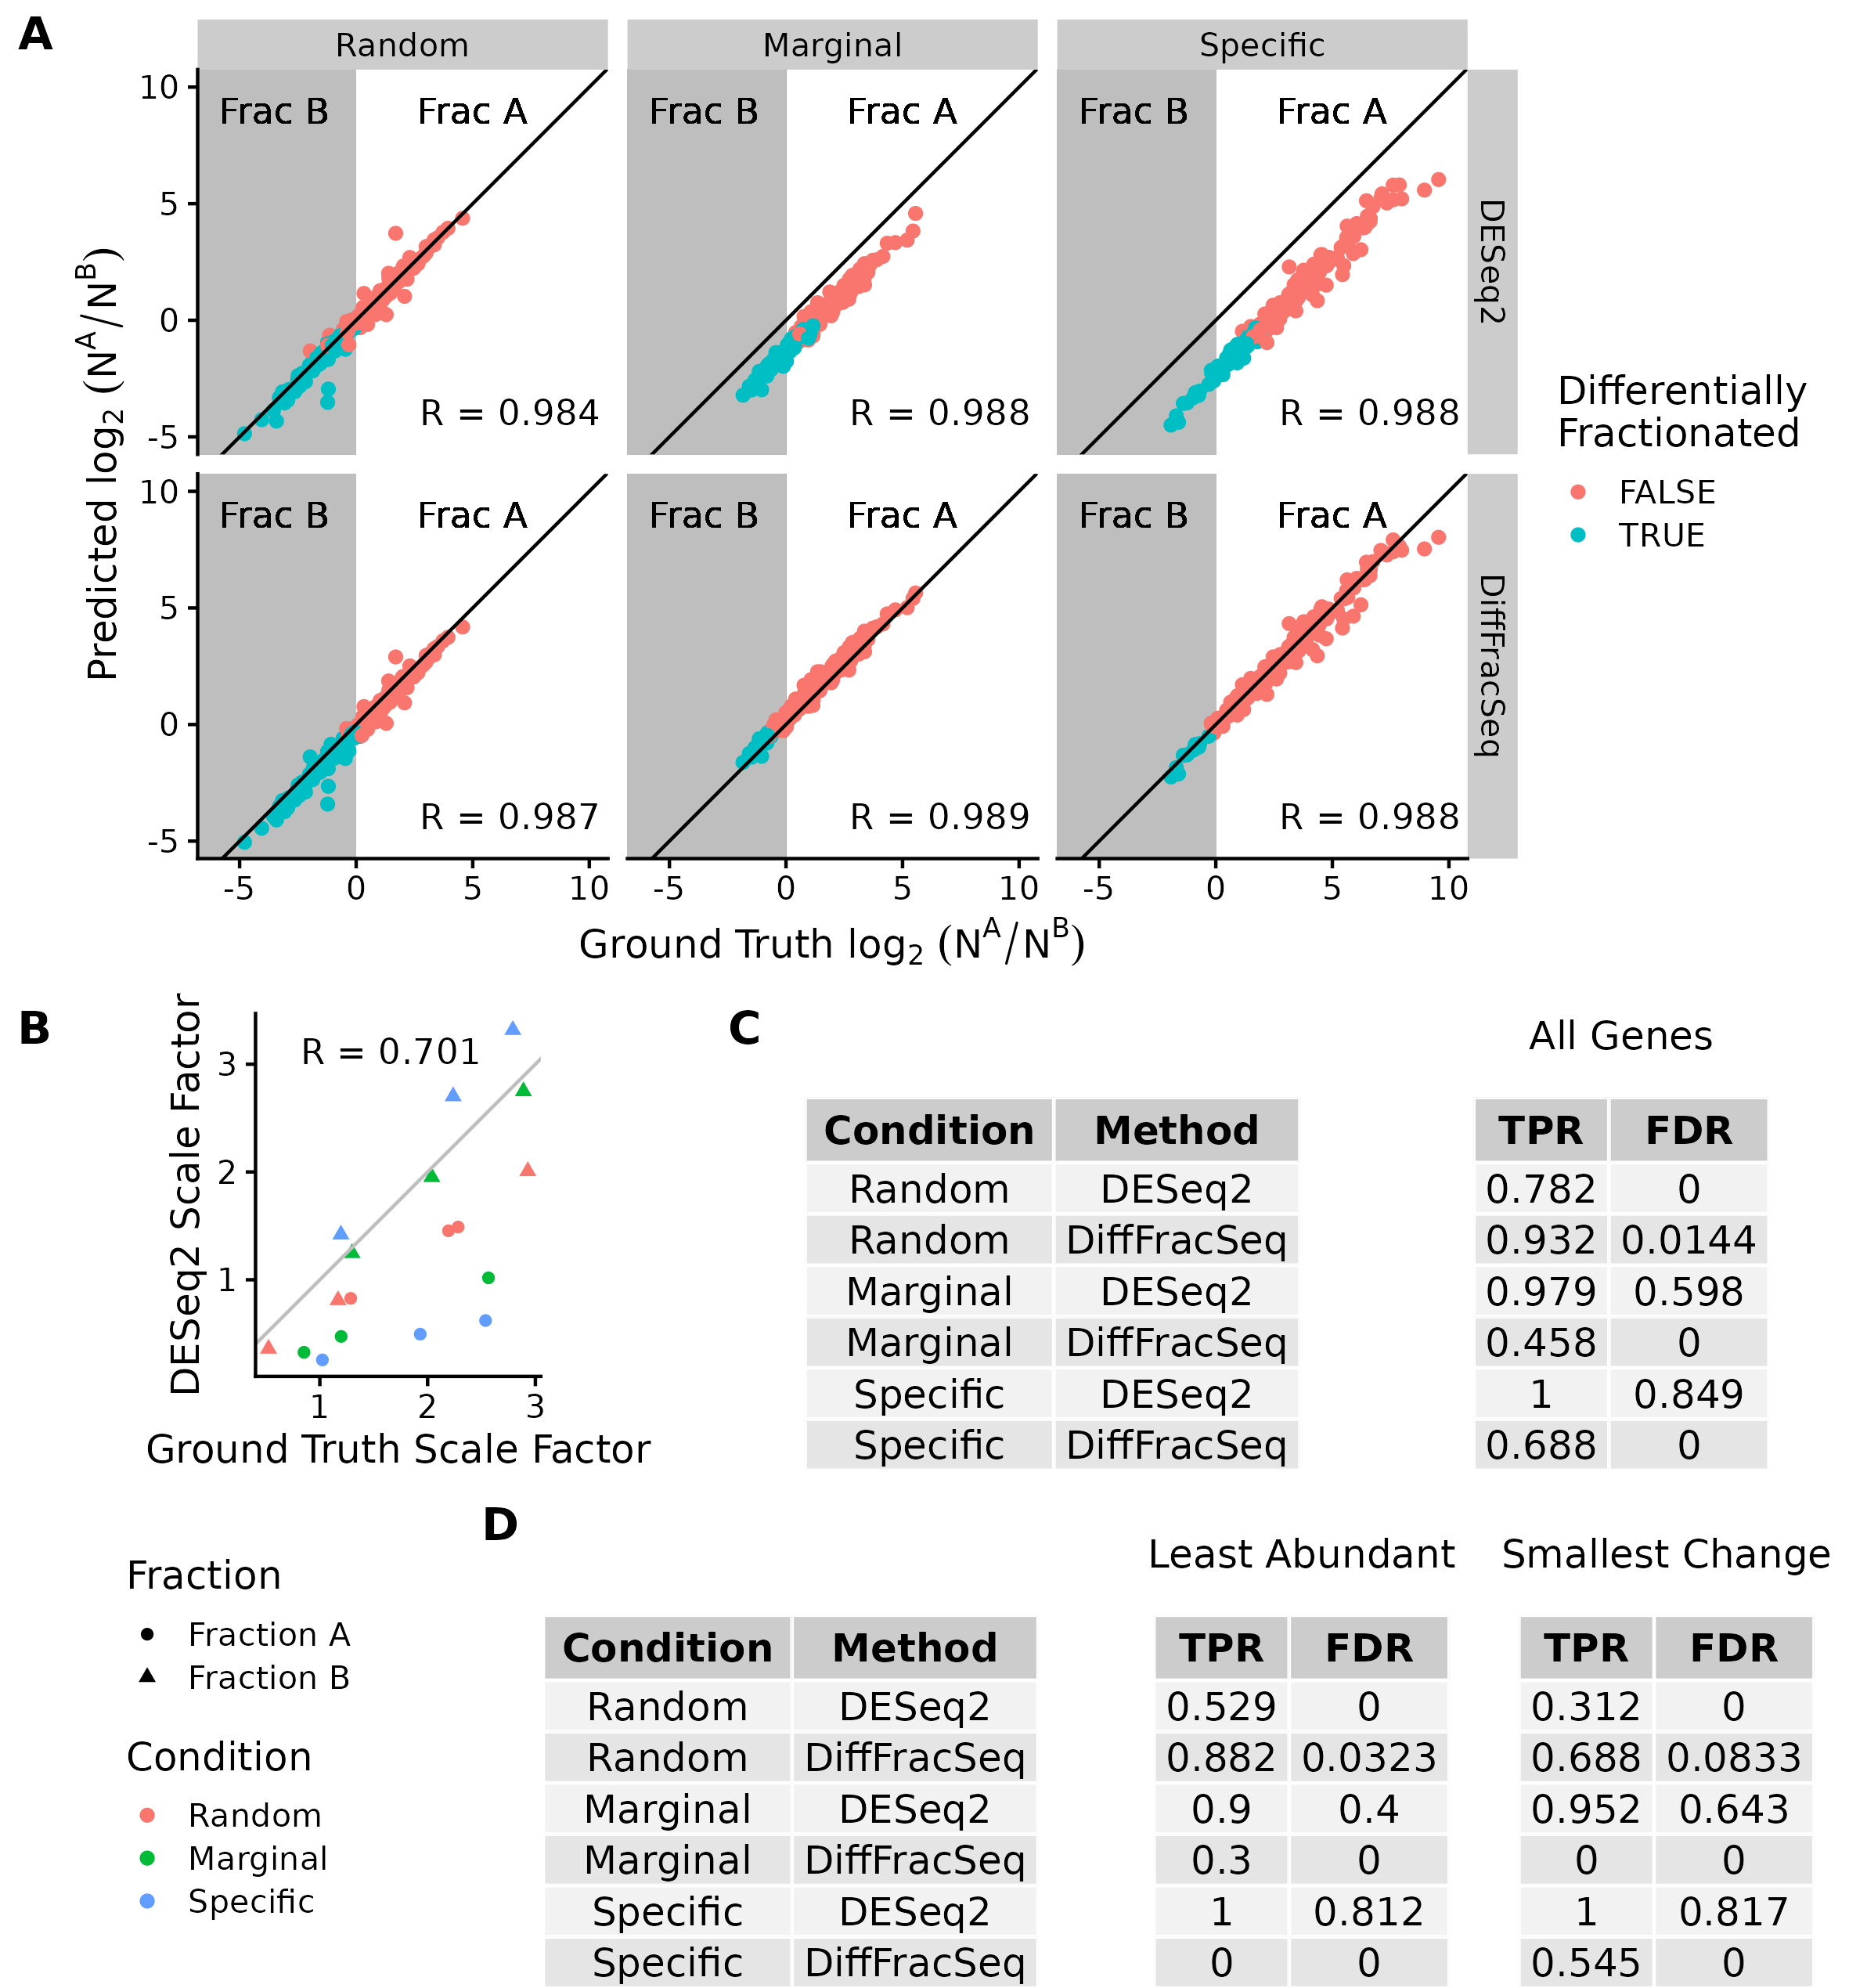
\includegraphics[width=1\linewidth]{figures/DESeq_vs_bayesian_combined.png} 

}

\caption[Simulated data performance.]{\textbf{Comparison of DESeq2 and DiffFracQuant performace a simulated data set.}} \label{fig:simulated-data-results}
\end{figure}

\subsection{Quantifying Fractionation in the Experimental Data Sets}

The performance of DiffFracQuant compared to DESeq2 was then checked using the ENCODE nuclear vs cytoplasmic fraction data set. 
Similar to the results from the simulated data set, the correlation in log$_2$ fraction ratios between the two methods is high, but only DiffFracQuant is able to suggest an asymmetric distribution in total transcript counts between the two fractions, \ref{fig:encode-iserman-data-results}A.
DiffFracQuant determines that the majority of poly(A) tailed RNA transcripts are found in the cytoplasm as expected in an unstressed sample of cells grown in standard conditions.
Over half of the 234 genes that DiffFracQuant detects as having transcripts localised to the nucleus are associated with roles other than protein coding, according to the PANTHER database. 
These genes are also detected to be differentially fractionated by DESeq2 alongside 4708 others, 3471 of which are known to be protein coding.
The ENCODE data set was also used to investigate DiffFracQuant's ability to analysis data sets that do not contain any replicates. 
A case which is DESeq2 is unable to analysis.
The results between using one and two replicates are correlated, $R = 0.84$, but there are quite significant differences in the number of genes that are determined to be differentially expressed, especially in low abundant genes, \ref{fig:encode-iserman-data-results}B.

\begin{figure}[h]

{\centering 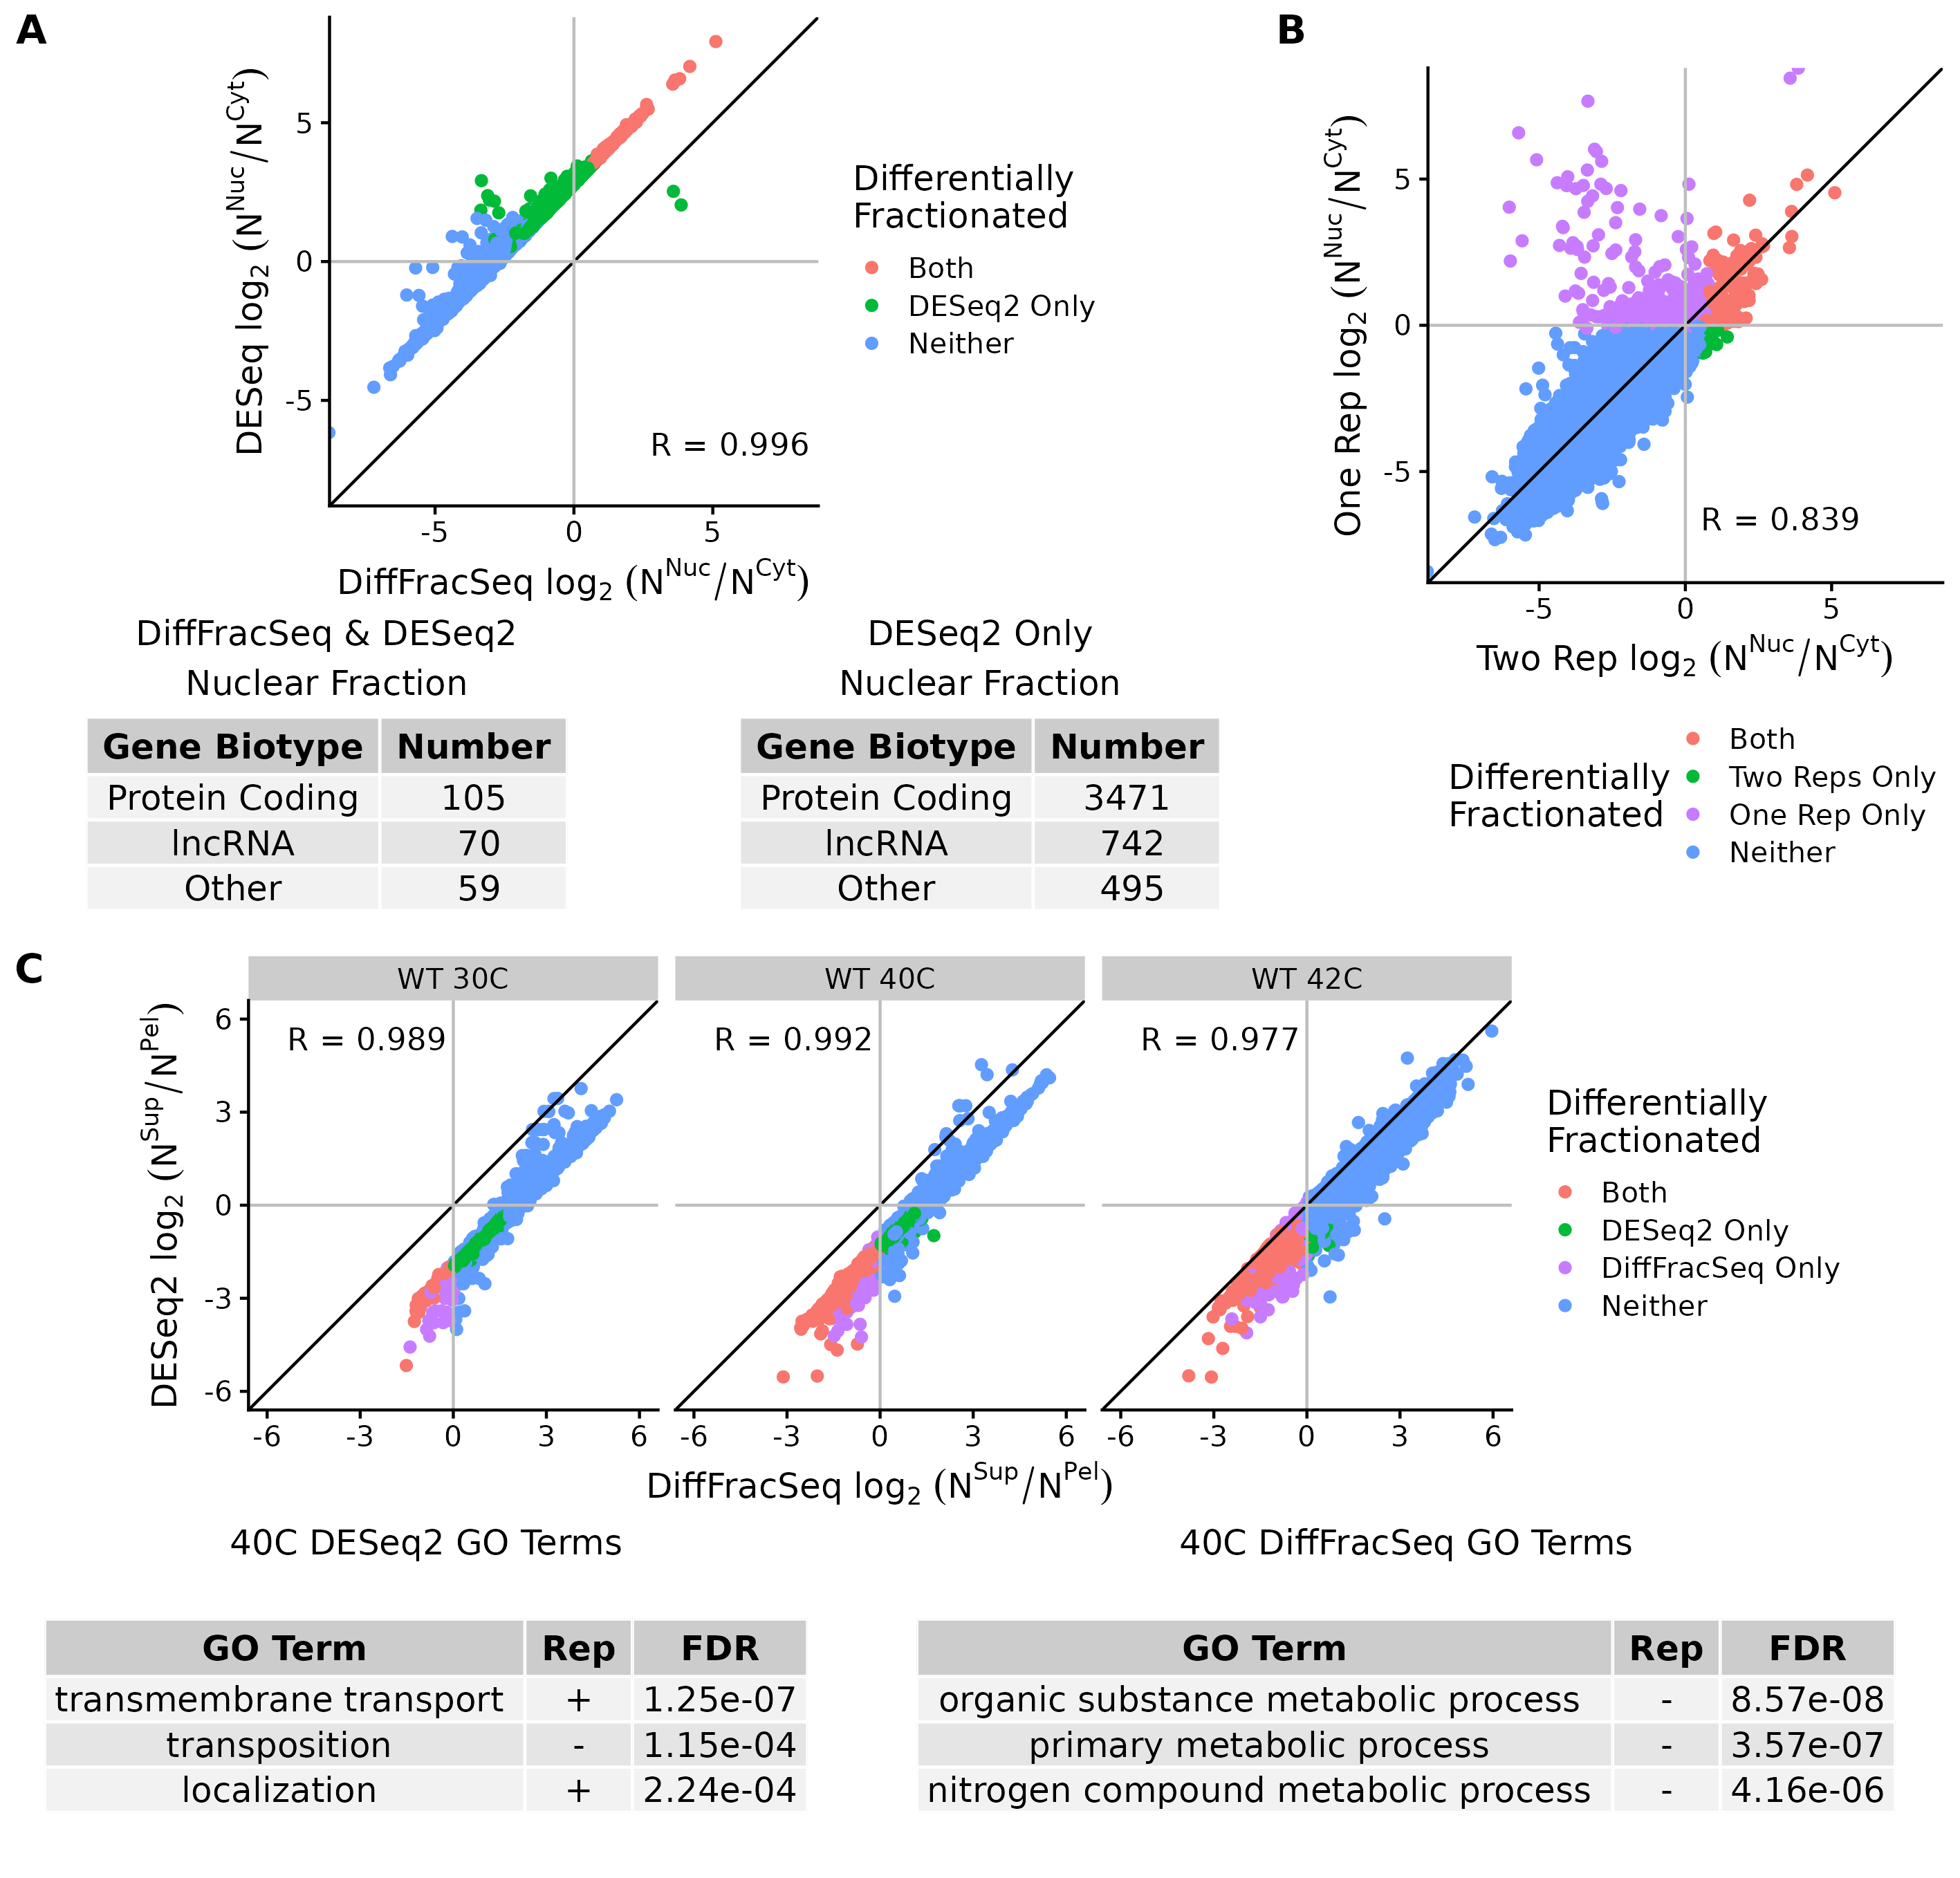
\includegraphics[width=1\linewidth]{figures/DESeq_vs_bayesian_encode_and_iserman_combined.png} 

}

\caption[Experimental data performance.]{\textbf{Comparison of DESeq2 and DiffFracQuant performace on two experimental data sets.}} \label{fig:encode-iserman-data-results}
\end{figure}





\section{Chapter 5 Conclusion}


Alternatively, instead of investigating within cell fractions, entire libraries of synthetic constructs can be characterised by sorting pools of constructs by some desired characteristic, for example high protein fluorescence, and sequencing these fractions (3). 
Despite the development of multiple fractionation-based RNA-Seq assays, there are a limited number of statistical methods to analyse them. 

\end{document}